\documentclass[14pt]{article}

\usepackage[utf8]{inputenc}
\usepackage[T2A]{fontenc}
\usepackage[english,russian]{babel}

\usepackage{graphicx}
\usepackage{mathtools,amssymb}
\usepackage{amsmath}

\usepackage{hyperref}

\usepackage{subcaption}
% Generate dummy text
\usepackage{lipsum}  
\usepackage{array,multirow}
\usepackage{svg}
\renewcommand\thesubfigure{\asbuk{subfigure}}

\def \adl {adl/}

\begin{document}

\begin{figure}
	\centering
	\includegraphics[width=0.7\linewidth]{pic/screenshot001}
	\caption{Схема расчётной области}
	\label{fig:screenshot001}
\end{figure}
a
	Математическая модель:
\begin{equation}\label{mm}
	\beta V_p\frac{\partial p}{\partial t} = q + \sum_{i=1}^{N}T_i\left(p-p_i\right)
\end{equation}

\begin{equation}\label{mm1}
	\beta V_p\frac{p^{n+1} - p^n}{\Delta t} = q^{n+1} + \sum_{i=1}^{N}T_i\left(p_i^{n+1}-p^{n+1}\right) + T_a\left(p_a - p^{n+1}\right)
\end{equation}

\begin{equation}
	q^n = -w\left(p^n-p_w^n\right)
\end{equation}


\begin{equation}
	p^n = p_w^n - \frac{1}{w}q^n = p_w^n - w^*q^n 
\end{equation}

\begin{equation}
	\beta V_p \left(p^{n+1} - p^n\right) = q^{n+1}\Delta t + \sum_{i=1}^{N}T_i\left(p_i^{n+1}-p^{n+1}\right)\Delta t + T_a\left(p_a - p^{n+1}\right)\Delta t
\end{equation}
	
\begin{eqnarray*}\label{mm2}
	\beta V_p \left(p_w^{n+1} - p_w^n\right) - \beta V_p w^*\left(q^{n+1} - q^n\right) = \\
	= q^{n+1}\Delta t + \sum_{i=1}^{N} T_i \left({p_w}_i^{n+1}-p_w^{n+1}\right)\Delta t - 
	\sum_{i=1}^{N} T_i \left(w_i q_i^{n+1}-w q^{n+1}\right)\Delta t \\
	+  T_a\left(p_a - p_w^{n+1}\right)\Delta t + T_a w^* q^{n+1}
\end{eqnarray*}
\begin{equation*}
	v^* = \frac{1}{\beta V_p}
\end{equation*}


\begin{eqnarray*}\label{mm3}
 \Delta p_w^{n+1}  = w^*\left(q^{n+1} - q^n\right) 
	+ q^{n+1} v^* \Delta t
	+ v^* \sum_{i=1}^{N} T_i \left({p_w}_i^{n+1}-p_w^{n+1}\right)\Delta t + \\
    - v^* \sum_{i=1}^{N} T_i \left(w_i^* q_i^{n+1}-w^* q^{n+1}\right)\Delta t 
	+  v^* T_a\left(p_a - p_w^{n+1}\right)\Delta t + v^* T_a w^* q^{n+1}
\end{eqnarray*}

\begin{eqnarray*}\label{mm4}
	p_w^{n+1} - p_w^m  = \underbrace{w^*\left(q^{n+1} - q^m\right) }_{1}
	+ \underbrace{\sum_{\tau=m+1}^{n+1}q^\tau v^* \Delta t }_{2}
	+\underbrace{v^* w^* \Delta t\left(\sum_{i=1}^{N} T_i + T_a \right)\sum_{\tau=m}^{n} q^\tau}_{3}\\
	+ v^* \sum_{\tau=m}^{n}\sum_{i=1}^{N} T_i \left({p_w}_i^\tau-p_w^\tau\right)\Delta t  
	- v^*  \sum_{\tau=m}^{n} \sum_{i=1}^{N} T_i w^*_i q_i^\tau \Delta t 
	+  \sum_{\tau=m}^{n} v^* T_a\left(p_a - p_w^\tau\right)\Delta t
\end{eqnarray*}



	$p$ - пластовое давление;
	
	$p_w$ - забойное давление;
	
	$q_m$ - массовый расход;
	
	$\sigma = \sigma(x,y)$ - гидропроводность;
	
	$\kappa_j$ - коэффициент связи с пластом для j-той скважины;
	
	$\lambda$ - продуктивность контура питания (аквифера).
	
	$m$ - пористость.
	
	$h$ - эффективная толщина.
	
\section{Результаты}	
	Алгоритмы восстановления пропусков:
	\begin{itemize}
		\item A1 --- Линейная интерполяция
		\item A2 --- Регрессия Дюпюи + компенскация
		\item A3 --- Локальный матбаланс
		\item A4 --- Линейная интерполяция пластовки, пеерсчёт на забойку
		\item A5 --- ADL
		\item A6 --- ADL + МП
	\end{itemize}

\begin{figure}
	\centering
	\includegraphics[width=0.9\linewidth]{pic/box_plot_all}
	\caption{Экзаменационная выборка}
	\label{fig:boxplotall}
\end{figure}
\begin{figure}
	\centering
	\includegraphics[width=0.9\linewidth]{pic/box_plot_train}
	\caption{Обучающая выборка}
	\label{fig:boxplottrain}
\end{figure}
\begin{figure}
	\centering
	\includegraphics[width=0.9\linewidth]{pic/box_plot_test}
	\caption{Тестовая выборка}
	\label{fig:boxplottest}
\end{figure}


\section{Алгоритм A4:}
Интерполяция забойного давления в предположении кусочно линейного изменения пластового давления с течением времени. Запишем уравнение Дюпюи в следующем виде:

\begin{equation}
	p^n = p_w^n - \frac{1}{w \tau^n}q^n = p_w^n - w^* \tau^{*n} q^n, 
\end{equation}
где $w$ -- продуктивность, $\tau$ -- коэффициент участия скважины. Для удобства записи будем использовать обратные значения $w^*$ и $\tau^{*n}$ соответственно.
\begin{equation*}
	\tau^n = \frac{h^n}{h^n_m},
\end{equation*}
где $h^n$ -- время работы скважины в часах, $h^n_m$ -- кол-во часов в месяце. 
С учётом инерционности изменения пластового давления, предположим что изменение пластового давления происходит линейно с течением времени. Полученную систему уравнений можно записать следующим образом:

\begin{equation}
	\begin{cases}
		p^n = p_w^n - w^*\tau^{*n}q^n 
		\\
		p^n = a_i*t^n+b_i
	\end{cases},
\end{equation}
где $i$ -- номер интервала. Систему уравнений исключив неизвестное значение $p^n$ можно преобразовать к виду:
 \begin{equation}
 	p_w^n = w^*\tau^{*n}q^n + a_i*t^n+b_i.
 \end{equation}
 Полученное уравнение имеет 3 неизвестных параметра, следовательно для их нахождения необходимо иметь как минимум 3 одновременных замера среднего расхода жидкости и забойного давления. Существующий временной ряд предлагается обрабатывать скользящим окном шириной в 3 замера. На рисунке \ref{fig:schimA4} схематически изображён принцип работы алгоритма.

\begin{figure}[!htb]
	\centering
	\includegraphics[width=1.0\linewidth]{screenshot001}
	\caption{Схема метода}
	\label{fig:schimA4}
\end{figure}

Полученный алгоритм был применено на Татсуксинском месторлождении, объект Тл.

\begin{figure}[!htb]
	\centering
	\includegraphics[width=1.0\linewidth]{pic/hist_mape_tat_a4}
	\caption{Погрешность настройки MAPE}
	\label{fig:MAPE_A4}
\end{figure}

\begin{figure}[!htb]
	\centering
	\includegraphics[width=1.0\linewidth]{pic/hist_rmse_tat_a4}
	\caption{Погрешность настройки RMSE}
	\label{fig:RMSE_A4}
\end{figure}

\begin{figure}[!htb]
	\centering
	\includegraphics[width=1.0\linewidth]{pic/cp_A2}
	\caption{Кроссплот}
	\label{fig:CP_A4}
\end{figure}

\begin{figure}[!htb]
	\centering
	\includegraphics[width=1.0\linewidth]{pic/pw_372g(13)_a4}
	\caption{Динамика давления и расхода жидкости скв. 372g}
	\label{fig:RMSE_A4_w1}
\end{figure}

скв. 372g
MAPE = 7.9\%, 3.9\%, 12.9\%
RMSE = 0.365, 0.142, 0.524 МПа


\begin{figure}[!htb]
	\centering
	\includegraphics[width=1.0\linewidth]{pic/pw_305u(3)_a4}
	\caption{Динамика давления и расхода жидкости скв. 305u}
	\label{fig:RMSE_A4_w2}
\end{figure}

скв. 305u
MAPE = 11.9\%, 7.9\%, 18.7\%
RMSE = 0.726, 0.620, 0.880 МПа


\begin{figure}[!htb]
	\centering
	\includegraphics[width=1.0\linewidth]{pic/pw_372g(13)_a4_stp2}
	\caption{Динамика давления и расхода жидкости скв. 372g ш2}
	\label{fig:RMSE_A4_w1}
\end{figure}


\begin{figure}[!htb]
	\centering
	\includegraphics[width=1.0\linewidth]{pic/pw_305u(3)_a4_stp2}
	\caption{Динамика давления и расхода жидкости скв. 305u ш2}
	\label{fig:pw305u3a4stp2}
\end{figure}


\section{Восстановление пропусков Гарейское тл}
На примере объекта разработки Гарейского месторождения Тл рассмотрим  работу алгоритма восстановления данных давления. Первый шаг алгоритма предполагает оценку пластовых и забойных давлений условно независимо для каждой скважины. Взаимовлияние скважин учитывается через усреднённое пластовое давление вблизи скважины.

\subsection{Математическая модель}
    Для решения задачи используем закон сохранения массы в виде уравнения материального баланса (МБ) и уравнение Дюпюи. 
    
\subsubsection{Использование уравнения материального баланса} Запишем уравнение МБ в конечно-разностном виде:
    
\begin{equation}\label{mb3}
	\begin{cases}
		\beta V_p\frac{p^{n+1} - p^n}{\Delta t} = q_w^{n+1} + q_a^{n+1} + q_b^{n+1},
		\\
		q_a^{n+1} = T_a \left(\alpha*\left(p_a - p^{n+1}\right) + \left(1-\alpha\right)\left(p_a - p^n\right)\right)
		\\
		q_b^{n+1} = T_b \left(\alpha*\left(p_b - p^{n+1}\right) + \left(1-\alpha\right)\left(p_b - p^n\right)\right)
		
	\end{cases}
\end{equation}
где $q_w$ -- среднемесячный расход жидкости на скважине, $q_a$ -- переток между контрольным объёмом и аквифером, $q_b$ -- переток между контрольным объёмом и окружающими пластом (контуром питания), $T_a$ -- проводимость аквифера, $T_b$ -- проводимость границы контура питания (между контрольным объёмом и окружающим пластом), $\bar{p}_b$ - усредненное давление на границе контрольного объёма (контуре питания скважины), $\alpha \in[0,1]$ -- коэффициент отвечающий за вид разностной схемы по времени (явной, полунеявной, неявной). При решении задаются граничные условия $p_a = p_0$ и начальное условие $p_b|_{t=0} = p_0$, где $p_0$ -- начальное пластовое давление.

Усреднённое давление на контуре питания находится по формуле:
\begin{equation}\label{mpc}
	\bar{p}_b = \frac{\mathrm{w}_p*\bar{p}_p + \mathrm{w}_i*\bar{p}_i + \mathrm{w}_s*\bar{p}_s}{\mathrm{w}_p + \mathrm{w}_i + \mathrm{w}_s},
\end{equation}
где $\mathrm{w}$ -- весовые коэффициенты для соответствующих средних давлений $\bar{p}$ добывающих, нагнетательных и остановленных скважин (индексы $p$, $i$ и $s$ соответственно). Весовые коэффициенты равны количеству скважин соответствующего типа на момент времени $n$. Усредненное давление находится опираясь на замеры на скважинах в ближайшем окружении от исследуемой.
Обычно в непосредственной близости от текущей скважины находится несколько соседних скважин. Обычно этого достаточно для того, чтобы оценить изменение среднего давления, если замеры выполняются регулярно. Однако частота замеров может не охватывать всю историю разработки. В таких случаях возможны пропуски данных в среднем давлении, их можно заполнить с помощью линейной интерполяции или интерполяции, основанной на решении уравнения МБ для группы скважин. С другой стороны, осреднение по группе скважин может приводить к появлению «выбросов» в некоторые моменты времени, которые объясняются либо вводом новых скважин в ранее не разбуренной зоне, имеющих давление, близкое к начальному пластовому, либо преобладанием в замерной выборке скважин одного типа (например, только нагнетательных). В этом случае необходимо проводить процедуру сглаживания или использовать в качестве интерполяционной модели модель МБ. 

\subsubsection{Использование уравнения Дюпюи}
С учётом технологических особенностей процесса разработки нефтяных месторождений, замеров забойного давления, как правило, заметно больше чем замеров пластового давления. Для более точной настройки модели можно использовать информацию о динамике изменения забойного давления. Связь забойного давления с пластовым для слабо сжимаемой жидкости описывается уравнением Дюпюи. Запишем уравнение Дюпюи в следующем виде:

\begin{equation}\label{dpi}
	p^n = p_w^n - \frac{1}{w \tau^n}q^n = p_w^n - w^* \tau^{*n} q^n, 
\end{equation}
где $w$ -- продуктивность, $\tau$ -- коэффициент участия скважины. Для удобства записи будем использовать обратные значения $w^*$ и $\tau^{*n}$ соответственно.
\begin{equation*}
	\tau^n = \frac{h^n}{h^n_m},
\end{equation*}
где $h^n$ -- время работы скважины в часах, $h^n_m$ -- кол-во часов в месяце.
В реальных условиях продуктивность скважины может меняться с течением времени. В качестве допущения предположим кусочно постоянный вид изменения продуктивности скважины с течением времени. В систему \ref{mb3} добавим уравнение \ref{dpi}. Добавление уравнения позволит увеличить объём выборки, тем самым потенциально позволит повысить точность получаемых решений.

\subsection{Решение обратной задачи} 
Для использования модели \ref{mb3} для расчёта пластовых давлений необходимо идентифицировать вектор содержащий 3 параметра: $[\beta V_p, T_a, T_b]$. Для их определения необходимо решить обратную задачу - минимизировать целевой функционал (ЦФ) характеризующий отклонение расчётных значений от фактических.
\begin{equation}\label{lf_min}
	LF(\boldsymbol{x_f}, \boldsymbol{x_c}, \boldsymbol{u})  \rightarrow min,
\end{equation}
где $\boldsymbol{x_f}$ и $\boldsymbol{x_f}$ -- фактические и расчётные значения, в целевую функцию могут входить ограничения на управляющие параметры $\boldsymbol{u}$.
 В зависимости от метода решения, ЦФ может включать дополнительные слагаемые, например, штрафные функции, которые обеспечивают реалистичность полученного результата. 
 
 В случае использования в качестве дополнительных опорных точек замеров забойного давления к решению обратной задачи добавляется ещё вектор параметров характеризующих продуктивность. С учётом того, что продуктивность скважины может меняться в процессе разработки по естественным или технологическим причинам, в условиях допущения о кусочно-линейном виде профиля продуктивности, количество параметров модели может заметно возрасти, искомый вектор будет иметь вид $[\beta V_p, T_a, T_b, \boldsymbol{WI}]$, где $\boldsymbol{WI}$ -- вектор параметров продуктивности, размерности равной количеству выделенных интервалов. При выборе количества интервалов важно найти баланс между точностью настройки модели и её способностью интерполировать данные.

\subsubsection{Методы решения: линейная регрессия} 
Обратную задачу \ref{lf_min} можно привести к виду множественной линейной регрессии и использовать хорошо разработанный инструментарий решения регрессионных задач. Приведем задачу \ref{mb3} к виду модели  авторегрессии и распределённого лага (ADL) \cite{econome3k}, где в качестве лага выступает зависимость пластового давления на текущем шаге от предыдущего.  
Уравнение \ref{mb3} преобразуем к виду:
\begin{equation}\label{mb3r1}
	p^{n+1} - p^n = \Delta p^{n,n+1} = v^*\sum_{\tau=m+1}^{n+1}q^{n+1}\Delta t + \lambda_a q_a^{n+1}\Delta t +	\lambda_b q_b^{n+1}\Delta t,
\end{equation}
где параметр $\lambda = \frac{T}{\beta V}$ для контура питания $b$ и аквифера $a$. С учётом отсутствия замеров давления для каждого месяца уравнение \ref{mb3r1} представим в виде:
\begin{equation}\label{mb3r2}
	\begin{aligned}
		\Delta p^{m,n+1} = v^* \sum_{\tau=m+1}^{n+1}q^{n+1}\Delta t + \lambda_a Q^{m,n+1}_a + \lambda_b Q^{m,n+1}_b,
		\\
		Q^{m,n+1}_a =  \lambda_a\left[\alpha\sum_{\tau=m+1}^{n+1} \left(p_a - p^{\tau}\right) + \left(1-\alpha\right)\sum_{\tau=m}^{n} \left(p_a - p^{\tau}\right)\right]\Delta t,
		\\
		Q^{m,n+1}_b =  \lambda_a\left[\alpha\sum_{\tau=m+1}^{n+1} \left(p_b^{\tau} - p^{\tau}\right) + \left(1-\alpha\right)\sum_{\tau=m}^{n} \left(p_b^{\tau} - p^{\tau}\right)\right]\Delta t,
	\end{aligned}
\end{equation}
где $Q^{m,n+1}_c$ и $Q^{m,n+1}_a$ -- оценки суммарного объёма обмена жидкостью с контуром питания и аквифером соответственно за интервал времени  $[m,n+1]$, $p^{\tau}$ -- приближенная оценка пластового давления в расчётной области в момент времени $\tau$. В первом приближении её можно найти линейно интерполируя известные значения в соседних точках, получим:
\begin{equation*}
	p^{\tau} = \frac{p^n - p^m}{n-m}\left(\tau-m\right) + p^m.
\end{equation*}
Пропущенные значения для $p_b$ также в первом приближении находятся при помощи линейной интерполяции. 
 Таким образом, с учётом указанных допущений для настройки модели необходимо определить 3 параметра $[v^*$, $\lambda_c$, $\lambda_a$]. 
 
Подставим уравнение \ref{dpi} в \ref{mb3r2}, получим:
\begin{equation}\label{mb3r3}
	\Delta p_w^{m,n+1} = w_k^* \left(\tau^{*n} q^n - \tau^{*m} q^m \right) + 
	 v^* \sum_{\tau=m+1}^{n+1}q^{n+1}\Delta t + \lambda_b Q^{m,n+1}_b + \lambda_a Q^{m,n+1}_a,
\end{equation}
где  $w_k^*$ -- обратное значение продуктивности скважины для временного интервала $k$.
Следовательно, для настройки модели, теперь необходимо определить 3+$k$ параметра $[v^*, \lambda_c, \lambda_a, \boldsymbol{w}^*_k]$. Использование замеров забойного давления целесообразно при их достаточном количестве. 

Имея достаточное количество уравнений \ref{mb3r3}, можно найти искомый вектор неизвестных параметров инструментами линейной регрессии. Систему уравнений можно представить в виде:
\begin{equation}\label{smb3r3}
\boldsymbol{\Delta p} = \boldsymbol{X} \boldsymbol{u},
\end{equation}
где $\boldsymbol{\Delta p}$ -- вектор разницы давлений для разных временных шагов, $\boldsymbol{X}$ -- матрица факторов, $\boldsymbol{u}$ -- вектор параметров. 
Расчёт искомого вектора $\boldsymbol{u}$ можно выполнять используя широко развитый инструментарий решения регрессионных задач используя, например, методы МНК, робастной регрессии, L1, L2 регуляризации и т.д..

После нахождения параметров подставляем их в прямую задачу \ref{mb3r1} и с требуемым шагом по времени (мес, квартал) находим расчётные значения пластового давления для всего временного интервала. С учётом того, что решение системы \ref{smb3r3} позволяет найти параметры, которые позволяют описать разницу давлений, полученное решение описывает тенденцию (тренд) изменения давления и в ряде случаев может давать сдвинутые абсолютные значения давления. Для корректировки абсолютных значений решается дополнительная задача -- подбирается коэффициент смещения для абсолютных значений. Искомый параметр можно найти по формуле:
\begin{equation}\label{shift}
	 b_{sh} = \sum_{ \tau=1}^{N}\mathrm{w_{sh}}^\tau\left(p^{\tau}_f - p^{\tau}_c \right),
\end{equation}
где $\mathrm{w_{sh}}^\tau$ -- весовой коэффициент характеризующий степень доверия к величине отклонения, позволяет снизить влияние «выбросов».

\subsubsection{Методы решения: оптимизационная постановка}
Задачу \ref{lf_min} можно решать в оптимизационной постановке используя разнообразные пакеты для решения оптимизационных задач. В этом случае целевую функцию необходимо записать в виде:
\begin{equation}\label{Jlf_min}
	J = \sum_{ \tau \in N}\mathrm{w}_p^{\tau}\left(p^{\tau}_f - p^{\tau}_c \right) +
	\sum_{ \tau \in M}\mathrm{w}_{p_w}^{\tau}\left({p_w}^{\tau}_f - {p_w}^{\tau}_c \right) +  
	J_{pnl},
\end{equation}
где $\mathrm{w}_p^{\tau}$ и $\mathrm{w}_{p_w}^{\tau}$ -- весовые коэффициенты характеризующие степень доверия к замеру, $N$ и $M$ -- множества моментов времени в которых есть замеры давления, $J_{pnl}$ -- слагаемое отвечающее за штрафные функции.
\begin{equation}\label{Jpnl}
	\begin{split}
	J_{pnl} = \sum_{\tau = 1}^{T}f_{lb}(p^{\tau}_c, p_{lb}) +
			   \sum_{\tau = 1}^{T}f_{ub}(p^{\tau}_c, p_{ub}) + 
			   \sum_{\tau = 1}^{T}f_{lb}({p_w}^{\tau}_c, {p_w}_{lb}) + \\
			   \sum_{\tau = 1}^{T}f_{ub}({p_w}^{\tau}_c, {p_w}_{ub}) +  
			   \sum_{\tau \in M}f_{lb}\left(sg^{\tau} \left(p^{\tau}_c - {p_w}^{\tau}_f \right), \Delta p_{lb}\right),
	\end{split}
\end{equation}
где $f_{lb}$ и $f_{ub}$ -- функции активации для учёта нижнего $lb$ и верхнего $ub$ ограничения. Функция представляет собой половину ветви параболы (при использовании квадрата отклонения в качестве функции потерь). Последние слагаемое устанавливает минимальную депрессию/репрессию $\Delta p_{lb}$ (разницу между забойным и пластовым давлением). Здесь $sg^{\tau}$ — коэффициент, учитывающий тип скважины в момент времени $\tau$ и равный 1 для добывающей скважины и -1 для нагнетательной скважины. Значения $p_{lb}$, $p_{ub}$, ${p_w}_{lb}$, и ${p_w}_{ub}$ представляют собой нижнее и верхнее ограничения допустимых значений для пластового и забойного давлений.

Значения $p^{\tau}_c$, ${p_w}^{\tau}_c$ получаются в результате решения прямой задачи \ref{dpi} и \ref{mb3r1}. Далее в зависимости от используемого метода возможно нахождение градиента ЦФ. В результат работы оптимизационного алгоритма находится искомые параметры. 

\subsubsection{Методы решения: сопоставление}
Решение может быть получено любым из описанных методов, однако все они имеют как преимущества так и недостатки. 
Преимущества методов, основанных на решении линейной регрессии, включают:
\begin{itemize}
	\item нахождение глобального минимума;
	\item решение, как правило, является прямым или итеративным, но с легко вычисляемым градиентом;
	\item по виду матрицы фактор можно сделать выводы о полученном решении (возможность получения решения, точность).
\end{itemize}

К недостаткам их использования можно отнести:
\begin{itemize}
 	\item сложность задания ограничений на параметры и фазовые переменные;
 	\item полученные значения параметров могут быть трудно интерпретируемыми;
 	\item не каждую разностную схему можно свести к уравнению вида линейной регрессии.
\end{itemize}


Преимущества методов, основанных на обобщённом решении оптимизационной задачи, заключаются в следующем:
\begin{itemize}
	\item простой учёт ограничений как на управляющие параметры так и на фазовые переменные;
	\item получение решения при минимальном количестве фактических замеров;
	\item прямая интерпретация параметров;
\end{itemize}

К недостаткам использования этих методов можно отнести:
\begin{itemize}
	\item вероятность нахождения локального минимума, срабатывания ограничения используемого метода;
	\item зависимость от начального приближения;
	\item необходимость итеративного решения. 
\end{itemize}
В предлагаемом алгоритме используются оба метода, выбирается решение наилучшее с точки зрения ЦФ. 

\subsection{Автоматизированное определение количества интервалов с постоянным значением продуктивности}
Изменение продуктивности скважины как правило приводит к заметному изменению расхода жидкости при постоянной депрессии или к изменению депрессии при фиксированных отборах. Следовательно, моменты изменения продуктивности можно фиксировать по заметному изменению этих показателей. 

\subsubsection{На основе расхода жидкости}
На первом шаге, с учётом не полного объёма данных необходимых для расчёта депрессии, основным показателем является  существенные продолжительное изменения дебита (приёмистости) жидкости.

 На рисунке \ref{fig:VisvalingamWhyatt_examp} представлен пример получения интервалов для кусочно-постоянной продуктивности. Исходной информацией является расход жидкости на скважине (синяя кривая), строится кривая накопленного расхода (серая линия). Использование накопленного значения помогает сгладить колебания исходной кривой. Это также позволяет определить интервалы с относительно постоянным расходом исходной кривой по точкам изгиба (красные точки).
 \begin{figure}[!htb]
	\centering
	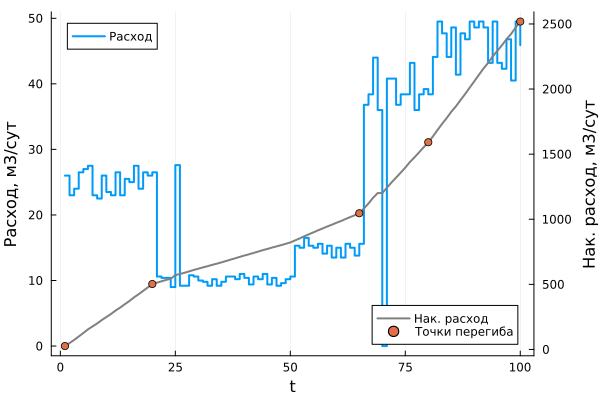
\includegraphics[width=20pc]{pic/VisvalingamWhyatt}
	%\includesvg[scale=1.0\linewidth]{pic/gar_cp.svg}
	\caption{Пример разбиения на интервалы на основе изменения расхода жидкости}
	\label{fig:VisvalingamWhyatt_examp}
\end{figure}
Поиск точек изгиба выполняется при помощи алгоритма Висвалингама–Уайатта \cite{VisWhy}. как видно из рисунка алгоритмом были найдены 3 из 4 моментов изменения расхода жидкости (красные точки). Использование накопленных значений позволяет также избежать реакции алгоритма на сильные единичные изменения расхода (выбросы). Таким образом использование представленного алгоритма позволяет предварительно оценить количество  интервалов с условно постоянными значениями продуктивности, и определить количество неизвестных параметров.

\subsubsection{На основе расхода жидкости и расчётного пластового давления}
На втором шаге, с учётом известной восстановленной динамики пластового давления, автоматизированное разбиение происходит путём объединения соседних временных шагов. Объединение происходит при помощи «жадного алгоритма», который в первую очередь объединяет интервалы, дающие минимальный прирост ошибки в итоговый целевой функционал.
\begin{enumerate}
	\item Для моментов времени с известными значениями забойного давления, рассчитываются значения продуктивности из формулы \ref{dpi}; 
	\item Отфильтровываются нефизичные значения продуктивности, рассчитывается целевая функция, характеризующая отклонение расчётных значений от фактических;
	\item Выполняется объединение с соседним интервалом, для объединённых интервалов рассчитывается общая продуктивность;
	\item Рассчитываются забойные давления, рассчитывается прирост ЦФ для каждого объединенного интервала;
	 \item Выбирается вариант объединения дающий минимальный прирост ЦФ;
	 \item Если количество интервалов больше 1, переход к п.3 
	 \item Строится график зависимости ЦФ от варианта объединения, "правилом локтя" выбирается вариант объединения.
\end{enumerate}
На рисунке \ref{fig:cJ11} представлен характерный вид зависимости ЦФ от варианта объединения. Красным кружком отмечен выбранный вариант объединения.
\begin{figure}[!htb]
	\center{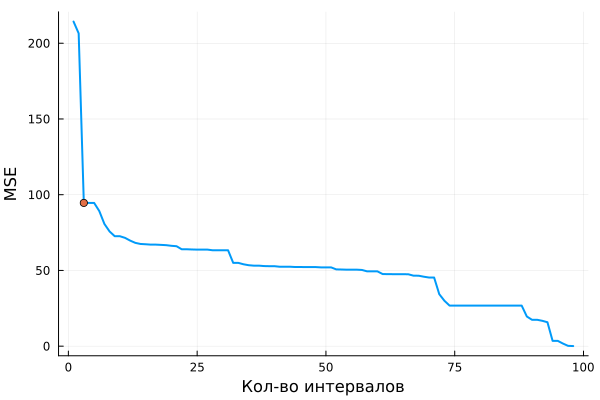
\includegraphics[width=20pc]{pic/cJ11}}
	\caption{График зависимости ЦФ от кол-ва интервалов}
	\label{fig:cJ11}
\end{figure}
Из графика видно, что зависимость ошибки от количества объединённых интервалов не является линейной. Максимальный рост ошибки происходит, когда все интервалы объединяются в несколько.
Объединение интервалов уменьшает количество настраиваемых параметров модели и улучшает её прогнозные (интерполяционные) свойства. Однако объединение всех интервалов в один не позволит упрощенной модели точно описать реальное взаимное изменение расхода жидкости и депрессии. 

\subsection{Тестирование. Синтетический пример}
Протестируем разработанный алгоритм на примере синтетического объекта разработки. В качестве исходной синтетической модели взята однофазная фильтрационная модель слабосжимаемой жидкости. Размер расчётной области 1000м. х 1000м. см. рис. \ref{fig:map9}. Расчётная сетка - прямоугольная, 441 расчётная ячейка. Шаг по времени 1 мес, период моделирования 100 месяцев.
\begin{figure}[!htb]
	\center{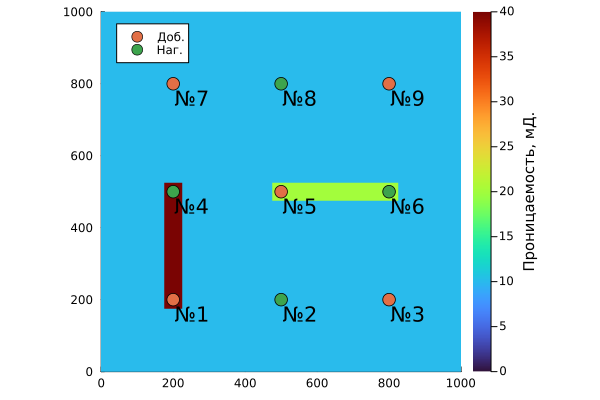
\includegraphics[width=20pc]{pic/map9sim1}}
	\caption{Схема расчётной области}
	\label{fig:map9}
\end{figure}
Моделируемый объект разрабатывается 9-ю скважинами (девятиточечная схема разработки), на скважинах задаются расходы жидкости в виде кусочно постоянных значений. Значения расхода и длительность периодов постоянства генерируются случайным образом. По периметру расчётной области поддерживается постоянное давление 20МПа. При помощи численной модели рассчитываются значения пластового и забойного давления вблизи скважин. 

В результате прямого моделирования был получен набор данных содержащий пластовые и забойные давления для всех скважин в каждый момент времени. Для каждой скважины набор данных был разделён на обучающую и тестовую выборки. Для пластового давления обучающая выборка составляла 10\% от всего объёма доступных данных, тестовая --- 90\% соответственно. Для забойного давления доля обучающей и тестовой выборок составлял по 50\%. Подобные соотношение характерно для практики.
На данные из обучающих выборок настраивалась модель \ref{mb3r2}, \ref{mb3r3}. Результаты настройки моделей для всех скважин представлены в таблице \ref{tabl:m9_well_m3k}. 

\begin{table}[!htb]
	\caption{Метрики для периода адаптации и прогноза}	
	\label{tabl:m9_well_m3k}	
	\begin{center}
		\begin{tabular}{c|c|c|c|c||c|c|c|c}
			\hline
			\multirow{3}{*}{Скв. №} & \multicolumn{4}{c||}{Пластовое давление} & \multicolumn{4}{c|}{Забойное давление} \\\cline{2-9}
			& \multicolumn{2}{c|}{MAPE, \%} & \multicolumn{2}{c||}{RMSE, МПа} & \multicolumn{2}{c|}{MAPE, \%} & \multicolumn{2}{c|}{RMSE, МПа} \\\cline{2-9}
			& обуч. & тест. & обуч.&тест. & обуч. & тест. & обуч.&тест.\\
			\hline
			1 & 4,3 & 3,0 & 0,8 & 0,7 & 0,7 & 1,1 & 0,2 & 0,3 \\
			2 & 4,3 & 2,6 & 0,6 & 0,8 & 1,9 & 1,5 & 0,4 & 0,4 \\
			3 & 9,1 & 9,9 & 1,7 & 1,9 & 1,4 & 1,6 & 0,1 & 0,2 \\
			4 & 1,8 & 1,4 & 0,4 & 0,4 & 0,8 & 1,0 & 0,3 & 0,3 \\
			5 & 2,5 & 3,4 & 0,6 & 0,7 & 2,7 & 2,0 & 0,3 & 0,4 \\
			6 & 1,5 & 1,7 & 0,4 & 0,4 & 0,5 & 0,5 & 0,2 & 0,2 \\
			7 & 4,2 & 3,8 & 0,9 & 1,0 & 2,3 & 1,6 & 0,2 & 0,2 \\
			8 & 4,7 & 4,5 & 1,1 & 1,2 & 1,6 & 2,9 & 0,8 & 0,8 \\
			9 & 2,4 & 2,4 & 0,5 & 0,5 & 1,8 & 1,7 & 0,3 & 0,3 \\
			\hline
			
		\end{tabular}
	\end{center}
\end{table}

В качестве примера приведём динамику давления для скважины №5. На рисунке \ref{fig:m9_din_w5a} представлены фактические и расчётные кривые пластового и забойного давления, кругляшками отмечены значения давления из обучающей выборки, остальные значения выступали в качестве тестовой выборки.
\begin{figure}[!htb]
	\centering
	\begin{subfigure}[b]{0.9\linewidth}
		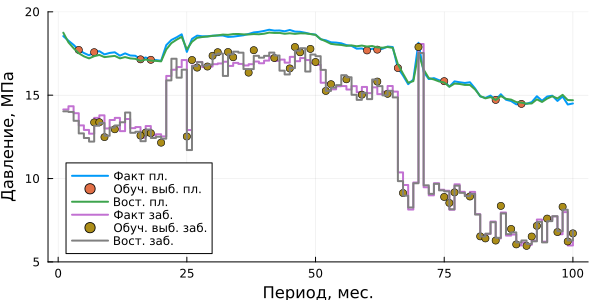
\includegraphics[width=\linewidth]{pic/simW5}
		\caption{}
		\label{fig:m9_din_w5a}
	\end{subfigure}
	\begin{subfigure}[b]{0.45\linewidth}
		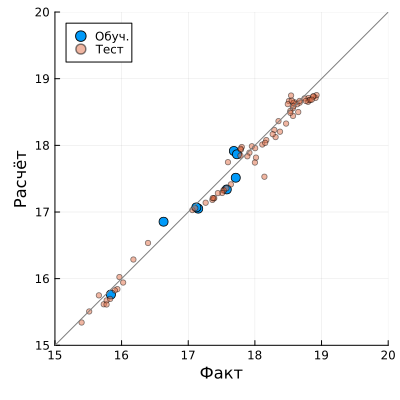
\includegraphics[width=\linewidth]{pic/cppplW5}
		\caption{}
		\label{fig:m9_din_w5b}
	\end{subfigure}
	\begin{subfigure}[b]{0.45\linewidth}
		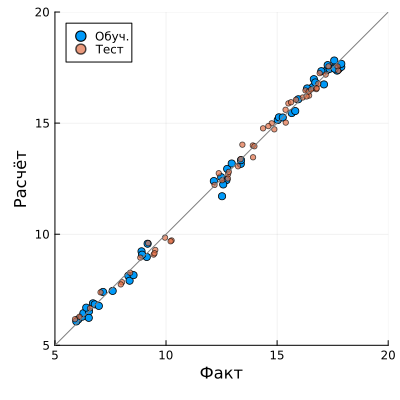
\includegraphics[width=\linewidth]{pic/cppwW5}
		\caption{}
		\label{fig:m9_din_w5c}
	\end{subfigure}
	\label{fig:m9_din_w5}
	\caption{Сопоставление фактических и расчётных значений давлений я для скважины №5, где (а) -- динамика, (б) -- кроссплот пластовое давление и (в) -- кроссплот забойное давление}
\end{figure}
На рисунках \ref{fig:m9_din_w5b} и \ref{fig:m9_din_w5c} показаны графики, на которых сопоставлены расчётные и фактические данные по пластовому и забойному давлению соответственно. Из этих графиков и таблицы можно сделать вывод, что модель с удовлетворительной точностью воспроизвела исходные данные.

\subsection{Тестирование. Гарейское Тл}
Применим разработанный подход к реальному объекту разработки. Объект разработки имеет 70 скважин, интенсивно разрабатывался с 2015 года. Обеспеченность замерами пластового давления  в среднем составляет 19,2\%. Обеспеченность замерами забойного давления в среднем составляет 55,9\%. Скважины обеспечены замерами неравномерно, гистограммы распределения обеспеченностью замеров представлены на рисунках \ref{fig:gar_hist_ppl_a} и \ref{fig:gar_hist_pw_b}. 
\begin{figure}[!htb]
	\begin{subfigure}[b]{0.45\linewidth}
		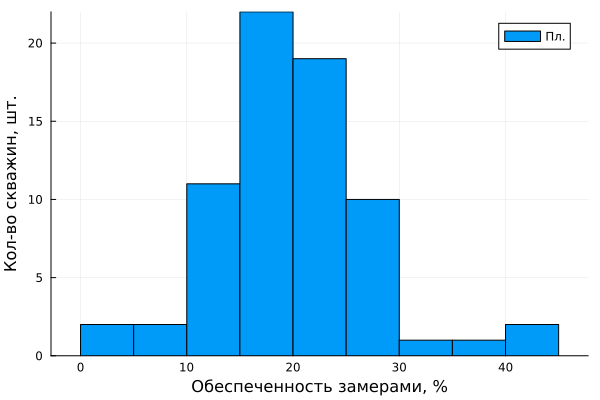
\includegraphics[width=\linewidth]{pic/hist_gar_ppl}
		\caption{}
		\label{fig:gar_hist_ppl_a}
	\end{subfigure}
	\begin{subfigure}[b]{0.45\linewidth}
		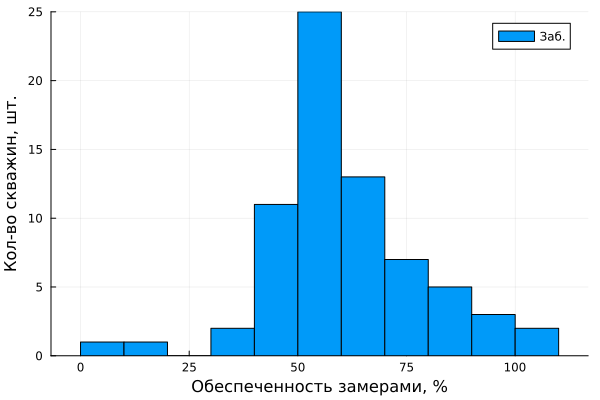
\includegraphics[width=\linewidth]{pic/hist_gar_pw}
		\caption{}
		\label{fig:gar_hist_pw_b}
	\end{subfigure}
	\label{fig:gar_hist}
	\caption{Гистограммы обеспеченности замерами пластового (а) и забойного давления (б)}
\end{figure}
Из рисунков видно, что часть скважин имеет очень низкую обеспеченность замерами, а некоторые скважины вообще не имеют замеров. Следует отметить что в представленной статистике участвуют как кондиционные так и не кондиционные замеры. Необходимо восстановить пропущенные значения, а также определить и исключить выбросы. 

Выполним восстановление пропущенных данных о пластовом давлении в два этапа.
На первом этапе используем всю доступную информацию для восстановления пропусков. На втором этапе исключим замеры, в которых отклонение фактического значения от расчётного превышает $3\sigma$. Затем повторим процедуру восстановления.
После восстановления пластового давления выполним восстановление забойного давления, используя автоматизированный подбор продуктивности в виде кусочно-постоянной функции.

На рисунке \ref{fig:cp_ppl_gar} представлен кроссплот, характеризующий отклонение фактических данных от расчётных. 
На рисунке \ref{fig:hist_ppl_gar} представлена гистограмма отклонения точки от диагонали (расстояние от точки до диагонали). 
\begin{figure}[!htb]
	\begin{subfigure}[b]{0.45\linewidth}
		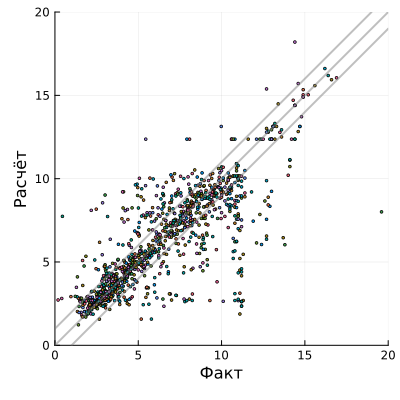
\includegraphics[width=\linewidth]{pic/gar_cp}
		\caption{}
		\label{fig:cp_ppl_gar}
	\end{subfigure}
	\begin{subfigure}[b]{0.45\linewidth}
		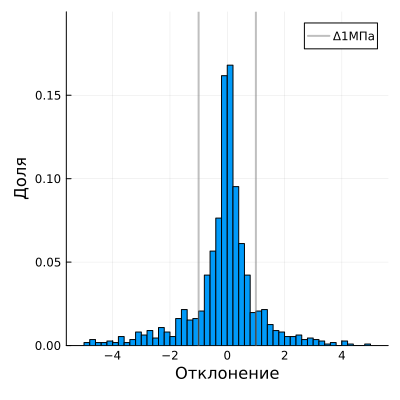
\includegraphics[width=\linewidth]{pic/gar_hg}
		\caption{}
		\label{fig:hist_ppl_gar}
	\end{subfigure}
	\label{fig:gar_er_ppl}
	\caption{Кроссплот (а) и гистограмма распределения отклонения значения от диагонали (б)}
\end{figure}
Из рисунков видно, что основной объём точек расположен вблизи диагонали и внутри полосы $\pm1МПа$. Точность настройки поскважинно можно представить в виде вертикальной гистограммы, на которой нанесено ранжированное по убыванию значение метрики MAPE для каждой скважины. Гистограммы представлены на рисунках \ref{fig:gar_tor_ppl_a} и \ref{fig:gar_tor_pw_b}.
\begin{figure}[!htb]
	\begin{subfigure}[b]{0.45\linewidth}
		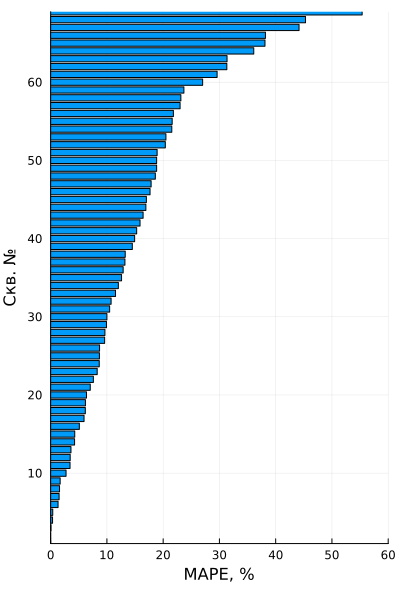
\includegraphics[width=\linewidth]{pic/tor_gar_ppl}
		\caption{}
		\label{fig:gar_tor_ppl_a}
	\end{subfigure}
	\begin{subfigure}[b]{0.45\linewidth}
		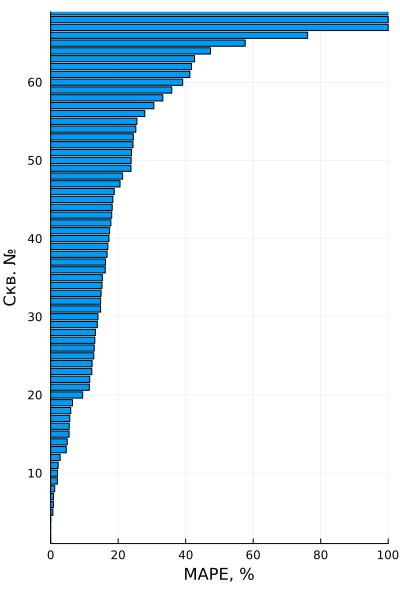
\includegraphics[width=\linewidth]{pic/tor_gar_pw}
		\caption{}
		\label{fig:gar_tor_pw_b}
	\end{subfigure}
	\label{fig:gar_hist}
	\caption{Гистограмма метрики MAPE по скважинам для пластового (а) и забойного (б) давления}
\end{figure}
Из рисунков видно, что около 70\% скважин для пластового и забойного давления имеют отклонение менее 20 и 25 \% соответственно. Стоит отметить, что большая величина отклонения может свидетельствовать не только о плохой настройке модели, но и о проблеме в качестве данных (выбросы, ошибки). Поэтому для скважин имеющих большое значение отклонение необходимо выполнить процедуру отбраковки/анализа данных повторно. 
Для настоящего объекта разработки отбраковка значений позволила исключить 57 замеров пластовых давлений и 83 замера забойного давления.
На рисунках \ref{fig:din_gar_press_11} и \ref{fig:din_gar_press_45} в качестве примера представлена динамика расчётного и фактического давления для скважин №11 и №45 соответственно. Отбракованные замеры (выбросы) на рисунке помечены чёрным крестиком. 
 \begin{figure}[!htb]
	\centering
	\begin{subfigure}[b]{0.9\linewidth}
	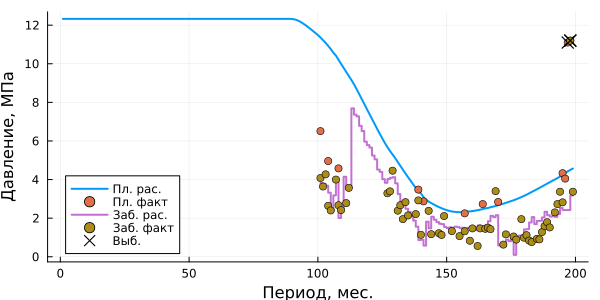
\includegraphics[width=1.0\linewidth]{pic/din_gar_press_11}
	%\includesvg[scale=1.0\linewidth]{pic/gar_cp.svg}
	\caption{}
	\label{fig:din_gar_press_11}
	\end{subfigure}
	\begin{subfigure}[b]{0.9\linewidth}
		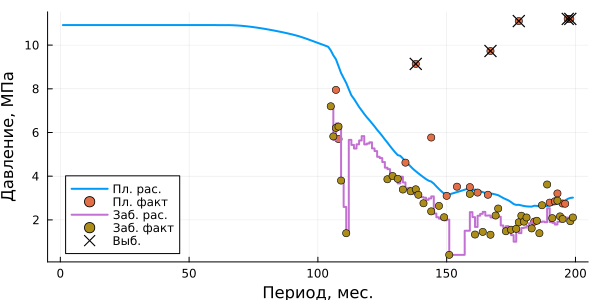
\includegraphics[width=\linewidth]{pic/din_gar_press_45}
		\caption{}
		\label{fig:din_gar_press_45}
	\end{subfigure}
		\caption{Динамика фактического и восстановленного давления для скв. №11 (а) и скв. №45 (б)}
\end{figure}
Отбраковка производится в автоматизированном режиме использовался метод "ящик с усами" \cite{BoxPlot}, где анализировалось отклонение замера от расчётной кривой, замеры имеющие значительное отклонение отбраковывались (присваивался весовой коэффициент 0). После чего процедура адаптации проводится ещё раз. 

Результатом работы алгоритма является динамика пластового и забойного давления для каждой скважины (для которой есть более 2-х замеров). Дополнительно отбраковываются замеры пластового и забойного давления отклонение которых от расчётных значений сильно превосходит основную массу замеров.

Представлена методика восстановления пропущенных значений замеров пластового и забойного давления на основе физически обоснованных зависимостей, таких как уравнение материального баланса и уравнение Дюпюи. Восстановление проводится индивидуально для каждой скважины, а влияние соседних скважин учитывается с помощью линейной аппроксимации средневзвешенного пластового давления близлежащих скважин. Методика была протестирована на синтетическом примере и применена для реального участка месторождения.

\newpage

\begin{thebibliography}{20}
		
		\bibitem{raf} R. Holanda, "A State-of-the-Art Literature Review on Capacitance
		Resistance Models for Reservoir Characterization
		and Performance Forecasting" Rafael Wanderley de Holanda, Eduardo Gildin, Jerry L. Jensen, Larry W. Lake and C. Shah Kabir. Energies 2018, 11(12), 3368; https://doi.org/10.3390/en11123368
		
		\bibitem{econome3k} Домбровский, В. В. Эконометрика: учебник / В. В. Домбровский. – М.: Новый учебник, 2004. – 342 с. - ISBN 5-8393-0400-X.
		
		\bibitem{kos} V. P. Kosyakov, "Structural and Parametric Identification
		of an Aquifer Model for an Oil Reservoir". Lobachevskii J. Math.
		{\bf 41}, 1242--1247 (2020).
		
		\bibitem{bas} K. S. Basniev, N. M. Dmitriev, R. D. Kanevskaya, and V. M. Maksimov,
		\textit{Underground hydromechanics}. M.-Izhevsk: Institute for
		Computer Research, 2006 [in Russian].
		
		\bibitem{azi} H. Aziz and E. Settari, \textit{Mathematical modeling of reservoir systems}.
		M.-Izhevsk: Institute for Computer Research, 2004 [in Russian].
		
		\bibitem{opt} V. P. Kosyakov and S. P. Rodionov, "Optimal control of wells on the basis
		of two-phase filtration equations", Proceedings of MIPT {\bf 8} (3),
		79--90 (2016).
		
		\bibitem{leg} V. P. Kosyakov and  D. Yu. Legostaev, "Using elements of machine learning to
		solve the inverse problem of reconstructing the hydraulic 
		conductivity feld for a fltration problem", Tyumen State University
		Herald. Physical and Mathematical Modeling. Oil, Gas, Energy {\bf 8}
		(2 (30)), 129--149.
		
		\bibitem{VisWhy}  Visvalingam, M.; Whyatt, J. D. (1993). "Line generalisation by repeated elimination of points" (PDF). The Cartographic Journal. 30 (1): 46–51. doi:10.1179/000870493786962263. ISSN 0008-7041.
		
		\bibitem{BoxPlot}  Сальникова Кристина Владимировна АНАЛИЗА МАССИВА ДАННЫХ С ПОМОЩЬЮ ИНСТРУМЕНТА ВИЗУАЛИЗАЦИИ «ЯЩИК С УСАМИ» // Universum: экономика и юриспруденция. 2021. №6 (81). URL: https://cyberleninka.ru/article/n/analiza-massiva-dannyh-s-pomoschyu-instrumenta-vizualizatsii-yaschik-s-usami (дата обращения: 11.09.2024).
		
\end{thebibliography}
	

	
\end{document}
